\chapter{المخططات الثنائية سائل--بخار والتقطير}\label{ch:b2:liquid-vapour-diagrams}

يحوّل إنبيق نحاسي نبيذًا فيه بضعة في المئة من الكحول إلى شراب أقوى منه
بأضعاف؛ وعمود التكرير يقسم النفط الخام إلى قطفاته، من الغاز إلى الفيول
الثقيل. وكلاهما يعتمد على حقيقة واحدة: البخار فوق خليط يغلي أغنى من السائل
بالمكوّن الأكثر تطايرًا. فإذا تكرر التبخير والتكثيف عددًا كافيًا من المرات
صار الفصل حادًا بالقدر المطلوب --- مع استثناء واحد: لا يوجد تقطير، مهما طال
العمود، يتجاوز بالإيثانول نحو 95 في المئة كتلةً. يرسم هذا الفصل
المخططات التي تبيّن كيف يغلي خليط من سائلين، ويستعملها في
تصميم عمود وفي معرفة الحد الذي يجب أن يتوقف عنده.

\begin{recall}
\Cref{ch:b2:chemical-potential}: \omterm{def:b2:chemical-potential:chemical-potential}{الجهد الكيميائي}، \omterm{thm:b2:chemical-potential:raoult}{وقانون راوول}
\omterm{def:b2:chemical-potential:ideal-mixture}{والخليط المثالي}، \omterm{def:b2:chemical-potential:activity-coefficient}{ومعاملات النشاطية} والانحرافات عن \omterm{thm:b2:chemical-potential:raoult}{قانون راوول}، وعلاقة
جيبس--دوهيم. \Cref{ch:b2:equilibrium-shifts}: \omterm{def:b2:equilibrium-shifts:variance}{التغايرية}. ومجلد
السنة الأولى، في التقنيات المخبرية: التقطير البسيط، والسوائل القابلة للامتزاج
وغير القابلة للامتزاج. والمجلد المدرسي: التقطير والتقطير المائي.
\end{recall}

\begin{omfigure}
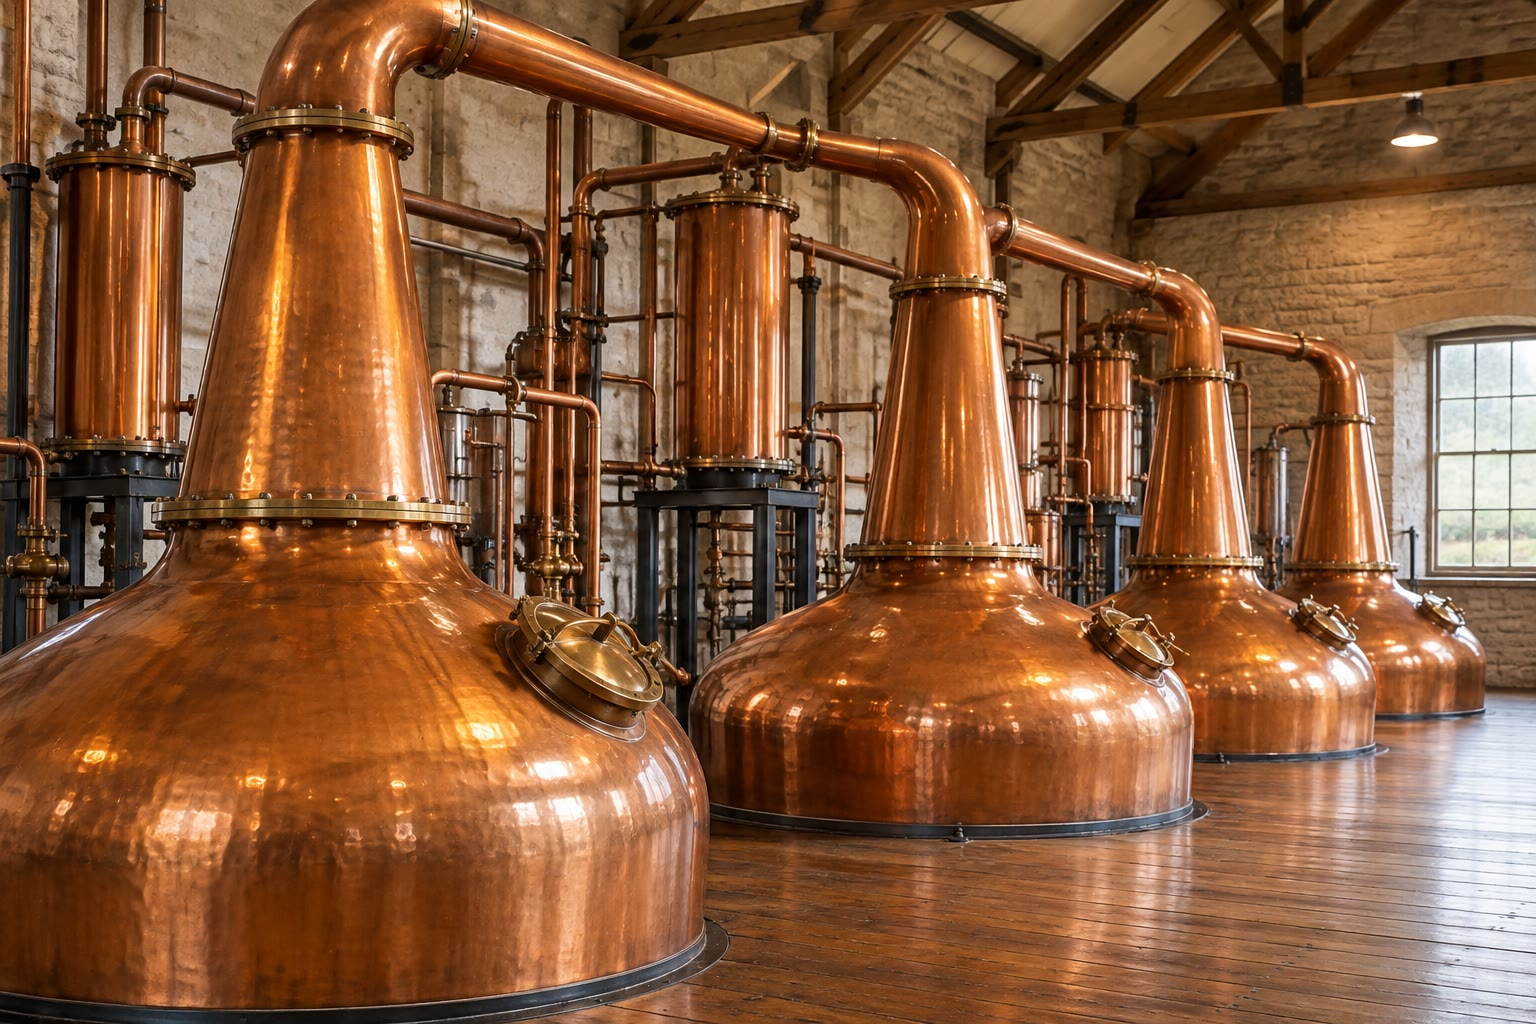
\includegraphics[width=0.62\linewidth]{images/book3/ai/b2-07-pot-stills.jpg}

{\small إنبيقات نحاسية في معمل تقطير. يُغلى كل شحن من المنقوع المخمَّر
ويُكثَّف بخاره: فيكون القطير الأول أغنى بالإيثانول بعدة أضعاف من المنقوع،
ويركّزه تقطير ثانٍ أكثر.}
\end{omfigure}

\section{الخلائط المثالية}

في هذا الفصل يُرقَّم السائلان 1 (الأكثر تطايرًا، ذو درجة الغليان
الأدنى) و2؛ و$x$ الكسر المولي للمكوّن 1 في السائل، و$y$ كسره
المولي في البخار، الذي يُعامل معاملة الغاز المثالي.

\begin{definition}[المخطط الثنائي]\label{def:b2:liquid-vapour-diagrams:binary-diagram}
\emph{المخطط الثنائي}\index{مخطط ثنائي} يبيّن، لخليط من مكوّنين،
الأطوار الموجودة وتراكيبها، بدلالة التركيب الإجمالي ومتغير
آخر واحد. و\emph{المخطط المتساوي الضغط}\index{مخطط متساوي الضغط} يُرسم في المستوي
(التركيب، درجة الحرارة) عند ضغط ثابت؛ و\emph{المخطط المتساوي
الحرارة}\index{مخطط متساوي الحرارة} في المستوي (التركيب، الضغط) عند
درجة حرارة ثابتة.
\end{definition}

\begin{definition}[منحنيا الفقاعة والندى]\label{def:b2:liquid-vapour-diagrams:bubble-dew}
على مخطط سائل--بخار، يعطي \emph{منحنى الفقاعة}\index{منحنى الفقاعة}
تركيب السائل في توازن مع البخار، ويعطي \emph{منحنى
الندى}\index{منحنى الندى} تركيب البخار في توازن مع السائل. ومن أجل
خليط معلوم التركيب عند ضغط ثابت، تكون \emph{نقطة
الفقاعة}\index{نقطة الفقاعة} هي درجة الحرارة التي تظهر عندها أول فقاعة
بخار عند التسخين، و\emph{نقطة الندى}\index{نقطة الندى} هي درجة
الحرارة التي تظهر عندها أول قطرة سائل عند تبريد البخار.
\end{definition}

\begin{proposition}[المنحنيات المثالية]\label{prop:b2:liquid-vapour-diagrams:ideal-curves}
من أجل \omterm{def:b2:chemical-potential:ideal-mixture}{خليط مثالي} عند درجة الحرارة $T$، حيث $p_1^*$ و$p_2^*$ ضغطا
بخار السائلين النقيين، يكون \omterm{def:b2:liquid-vapour-diagrams:bubble-dew}{منحنى الفقاعة} في \omterm{def:b2:liquid-vapour-diagrams:binary-diagram}{المخطط المتساوي الحرارة}
المستقيمَ $p = p_2^* + x(p_1^* - p_2^*)$، \omterm{def:b2:liquid-vapour-diagrams:bubble-dew}{ومنحنى الندى}
القطعَ الزائد
\[
  p = \frac{1}{y/p_1^* + (1 - y)/p_2^*} .
\]
\end{proposition}

\begin{proof}
يعطي \omterm{thm:b2:chemical-potential:raoult}{قانون راوول} الضغطين الجزئيين $p_1 = xp_1^*$ و$p_2 = (1 -
x)p_2^*$؛ ومجموعهما الضغط الكلي، الخطي في $x$. وفي البخار،
$y = p_1/p$، ومنه $x = yp/p_1^*$ و$1 - x = (1 - y)p/p_2^*$؛ وبالجمع،
$1 = p\,[y/p_1^* + (1 - y)/p_2^*]$.
\end{proof}

\begin{proposition}[البخار أغنى بالمكوّن الأكثر تطايرًا]\label{prop:b2:liquid-vapour-diagrams:richer}
من أجل \omterm{def:b2:chemical-potential:ideal-mixture}{خليط مثالي} فيه $p_1^* > p_2^*$ و$0 < x < 1$، يكون $y > x$.
\end{proposition}

\begin{proof}
$y = xp_1^*/p$ مع $p = xp_1^* + (1 - x)p_2^* < p_1^*$ لأن $p$
متوسط مرجَّح للمقدارين $p_1^*$ و$p_2^*$، يقع بينهما تمامًا. ومنه $y >
x$.
\end{proof}

\omterm{def:b2:liquid-vapour-diagrams:binary-diagram}{المخطط المتساوي الضغط} هو الذي يصف التقطير، الذي يجري عند الضغط
الجوي. وليست له صيغة بسيطة: فلكل درجة حرارة بين
نقطتي الغليان يُحسب $p_1^*(T)$ و$p_2^*(T)$ (هنا بمعادلة
أنطوان، $\log_{10}(p^*/\unit{bar}) = A - B/(T + C)$، المضبوطة على ضغوط
بخار مقيسة)، ثم تركيبا السائل والبخار اللذان
يعطيان ضغطًا كليًا قدره \qty{1.013}{bar}:
\[
  x = \frac{p - p_2^*(T)}{p_1^*(T) - p_2^*(T)}, \qquad y = \frac{x\,p_1^*(T)}{p} .
\]
لم يعد \omterm{def:b2:liquid-vapour-diagrams:bubble-dew}{منحنى الفقاعة} مستقيمًا؛ ويبقى \omterm{def:b2:liquid-vapour-diagrams:bubble-dew}{منحنى الندى} فوقه،
ويبقى البخار أغنى بالمكوّن الخفيف.

\begin{example}[البنزين والتولوين عند \qty{90}{\degreeCelsius}]\label{ex:b2:liquid-vapour-diagrams:benzene-toluene}
يكوّن البنزين والتولوين خليطًا شبه مثالي. وعند \qty{90}{\degreeCelsius}
تعطي معادلتا أنطوان $p_1^* = \qty{1.361}{bar}$ (البنزين) و$p_2^* =
\qty{0.542}{bar}$ (التولوين). وعند \qty{1.013}{bar}: $x = (1.013 - 0.542)/(1.361 -
0.542) = 0.575$ و$y = 0.575 \times 1.361/1.013 = 0.773$. فالسائل الذي فيه 57.5~\%
من البنزين (بالمولات) يغلي عند \qty{90}{\degreeCelsius} ويعطي بخارًا فيه
77~\%.
% ledger: antoine:benzene.A, antoine:benzene.B, antoine:benzene.C, antoine:toluene.A, antoine:toluene.B, antoine:toluene.C
\end{example}

\begin{omfigure}
\begin{tikzpicture}
\begin{axis}[omphase, width=0.47\linewidth, height=6cm, ymin=78, ymax=113,
  xlabel={\shortstack{\foreignlanguage{arabic}{$x$، $y$ (البنزين)}}}, ylabel={\babelsublr{$T$ (\unit{\degreeCelsius})}},
  title={\foreignlanguage{arabic}{\small متساوي الضغط، \qty{1.013}{bar}}}]
\addplot[omliquidus] table[x=x, y=T] {figdata/out/bachelor-2-liquid-vapour-a.dat};
\addplot[omsolidus] table[x=y, y=T] {figdata/out/bachelor-2-liquid-vapour-a.dat};
\draw[tieline] (axis cs:0.405,95) -- (axis cs:0.626,95);
\fill (axis cs:0.5,95) circle (1.3pt);
\draw[->, thick] (axis cs:0.5,82) -- (axis cs:0.5,104) node[above, font=\scriptsize] {تسخين};
\node[font=\scriptsize] at (axis cs:0.2,85) {سائل};
\node[font=\scriptsize] at (axis cs:0.85,108) {بخار};
\node[font=\scriptsize, omDef, anchor=north] at (axis cs:0.22,96) {الفقاعة};
\node[font=\scriptsize, omThm, anchor=south west] at (axis cs:0.62,101) {الندى};
\end{axis}
\end{tikzpicture}\hfill
\begin{tikzpicture}
\begin{axis}[omphase, width=0.47\linewidth, height=6cm, ymin=0.3, ymax=1.1,
  xlabel={\shortstack{\foreignlanguage{arabic}{$x$، $y$ (البنزين)}}}, ylabel={\babelsublr{$p$ (\unit{bar})}},
  title={\foreignlanguage{arabic}{\small متساوي الحرارة، \qty{80}{\degreeCelsius}}}]
\addplot[omliquidus] table[x=x, y=pbub] {figdata/out/bachelor-2-liquid-vapour-b.dat};
\addplot[omsolidus] table[x=x, y=pdew] {figdata/out/bachelor-2-liquid-vapour-b.dat};
\node[font=\scriptsize] at (axis cs:0.75,0.98) {سائل};
\node[font=\scriptsize] at (axis cs:0.2,0.36) {بخار};
\end{axis}
\end{tikzpicture}

{\small البنزين--التولوين، محسوبًا من \omterm{thm:b2:chemical-potential:raoult}{قانون راوول} ومعادلتي
أنطوان. يمينًا، عند الضغط الجوي: \omterm{def:b2:liquid-vapour-diagrams:bubble-dew}{منحنى الفقاعة} (بالأزرق) \omterm{def:b2:liquid-vapour-diagrams:bubble-dew}{ومنحنى الندى}
(بالأحمر)؛ فالسائل ذو التركيب 0.5 يبدأ بالغليان عند
\qty{92.1}{\degreeCelsius} ويصير كله بخارًا عند \qty{98.8}{\degreeCelsius}؛ وعند
\qty{95}{\degreeCelsius} (خط الربط المتقطع) ينقسم إلى سائل تركيبه 0.405
وبخار تركيبه 0.626. ويسارًا، عند \qty{80}{\degreeCelsius}: \omterm{def:b2:liquid-vapour-diagrams:bubble-dew}{منحنى الفقاعة}
مستقيم، \omterm{def:b2:liquid-vapour-diagrams:bubble-dew}{ومنحنى الندى} قطع زائد، والسائل الآن في الأعلى.}
% ledger: antoine:benzene.A, antoine:toluene.A (all six parameters in figdata/bachelor-2/liquid-vapour.py)
\end{omfigure}

\section{قراءة مخطط}

\begin{proposition}[تغايرية نظام ثنائي ذي طورين]\label{prop:b2:liquid-vapour-diagrams:variance}
لخليط من مكوّنين في طورين \omterm{def:b2:equilibrium-shifts:variance}{تغايرية} قدرها 2. فعند ضغط ثابت
تحدد درجة الحرارة وحدها تركيبي الطورين: ويُقرآن
عند طرفي القطعة الأفقية المارة بالنقطة الممثِّلة،
المسماة خط الربط.
\end{proposition}

\begin{proof}
المتغيرات المكثفة: $T$، و$p$، و$x$، و$y$. والعلاقات: تساوي الجهدين
الكيميائيين للمكوّن 1 وللمكوّن 2 بين الطورين. $v = 4 - 2 = 2$ (وقاعدة الأطوار
$v = n - r + 2 - \varphi$ تعطي النتيجة نفسها مع $n = 2$، $r = 0$، $\varphi = 2$).
وتثبيت $p$ يترك درجة حرية واحدة: $x(T)$ و$y(T)$ هما المنحنيان.
\end{proof}

\begin{theorem}[قاعدة الرافعة]\label{thm:b2:liquid-vapour-diagrams:lever}
خليط تركيبه الإجمالي $z$، منقسم إلى سائل تركيبه $x$
وبخار تركيبه $y$، يحوي كميتين $n_L$ من السائل و$n_V$ من
البخار بحيث
\[
  n_L\,(z - x) = n_V\,(y - z), \qquad \frac{n_V}{n_L + n_V} = \frac{z - x}{y - x} .
\]
هذه هي \emph{قاعدة الرافعة}\index{قاعدة الرافعة}: كل طور يكون أوفر
كلما اقترب تركيبه من التركيب الإجمالي، كالأثقال على
رافعة ترتكز عند $z$.
\end{theorem}

\begin{proof}
حفظ المكوّن 1: $(n_L + n_V)z = n_Lx + n_Vy$، ومنه $n_L(z - x) =
n_V(y - z)$؛ نقسم على $n_L + n_V$ ونعيد الترتيب.
\end{proof}

تصح \omterm{thm:b2:liquid-vapour-diagrams:lever}{قاعدة الرافعة} بالكسور المولية وكميات المادة، كما هنا، أو بالكسور
الكتلية والكتل: فالحفظ المستعمل واحد.

\begin{method}[قراءة مخطط ثنائي]\label{met:b2:liquid-vapour-diagrams:read-diagram}
\begin{enumerate}
  \item ضع النقطة (التركيب الإجمالي، درجة الحرارة) وسمِّ
        منطقتها: سائل، أو بخار، أو سائل + بخار.
  \item في منطقة ذات طورين، ارسم خط الربط المار بالنقطة؛ فطرفاه
        يعطيان تركيب السائل (على \omterm{def:b2:liquid-vapour-diagrams:bubble-dew}{منحنى الفقاعة}) وتركيب
        البخار (على \omterm{def:b2:liquid-vapour-diagrams:bubble-dew}{منحنى الندى}).
  \item استخرج نسب الطورين من \omterm{thm:b2:liquid-vapour-diagrams:lever}{قاعدة الرافعة}.
  \item لتتبع تسخين، حرّك النقطة نحو الأعلى: تظهر أول فقاعة
        على \omterm{def:b2:liquid-vapour-diagrams:bubble-dew}{منحنى الفقاعة}، وتختفي آخر قطرة على \omterm{def:b2:liquid-vapour-diagrams:bubble-dew}{منحنى الندى}؛
        وبينهما يزداد السائل فقرًا بالمكوّن الخفيف.
\end{enumerate}
\end{method}

\begin{example}[تبخير فجائي عند \qty{95}{\degreeCelsius}]\label{ex:b2:liquid-vapour-diagrams:flash}
يُرفع \qty{100}{mol} من خليط بنزين--تولوين متساوي المولات إلى
\qty{95}{\degreeCelsius} عند الضغط الجوي. يعطي خط الربط $x =
0.405$، $y = 0.626$؛ وكسر البخار $(0.500 - 0.405)/(0.626 - 0.405) =
0.43$: أي \qty{43}{mol} من البخار تحوي $43 \times 0.626 = \qty{27}{mol}$ من
البنزين، و\qty{57}{mol} من السائل تحوي \qty{23}{mol}. فمرحلة توازن واحدة
تُغني، لكن قليلًا فقط.
\end{example}

\section{الخلائط الحقيقية والأزيوتروبات}

حين تختلف \omterm{def:b2:chemical-potential:activity-coefficient}{معاملات النشاطية} عن 1 (\cref{ch:b2:chemical-potential})،
تبتعد الضغوط الجزئية عن مستقيمات راوول. فمع انحراف موجب
($\gamma > 1$: تتجاذب الجزيئات غير المتماثلة أقل مما تتجاذب
المتماثلة) يقع الضغط الكلي فوق الخط المثالي؛ ومع انحراف سالب
تحته. وإذا كان الانحراف قويًا بما يكفي، مرّ الضغط الكلي بقيمة
قصوى.

\begin{definition}[الأزيوتروب]\label{def:b2:liquid-vapour-diagrams:azeotrope}
\emph{الأزيوتروب}\index{أزيوتروب} خليط سائل يغلي دون أن
يتغير تركيبه: فالبخار الذي يعطيه له تركيبه نفسه. و\emph{الأزيوتروب
الموجب}\index{أزيوتروب موجب} (انحراف موجب) له
قيمة عظمى للضغط على \omterm{def:b2:liquid-vapour-diagrams:binary-diagram}{المخطط المتساوي الحرارة} وقيمة صغرى لدرجة الغليان
على \omterm{def:b2:liquid-vapour-diagrams:binary-diagram}{المخطط المتساوي الضغط}؛ و\emph{الأزيوتروب السالب}\index{أزيوتروب سالب}
بالعكس.
\end{definition}

\begin{theorem}[جيبس--كونوفالوف]\label{thm:b2:liquid-vapour-diagrams:konovalov}
على \omterm{def:b2:liquid-vapour-diagrams:binary-diagram}{مخطط ثنائي} سائل--بخار، عند قيمة قصوى للضغط الكلي (عند
درجة حرارة ثابتة) أو لدرجة الغليان (عند ضغط ثابت)، يكون للسائل
والبخار التركيب نفسه. وبالعكس، حيث يتساوى
التركيبان، يكون للمنحنيين مماس أفقي مشترك.
\end{theorem}

\begin{proof}[برهان عند درجة حرارة ثابتة]
علاقة جيبس--دوهيم للسائل عند $T$ ثابتة (مع إهمال الأثر الصغير للضغط $p$
على السائل) هي $x\,d\mu_1 + (1 - x)\,d\mu_2 = 0$. وعند التوازن
$\mu_i = \mu_i^\circ + RT\ln(p_i/p^\circ)$ مع $p_1 = yp$، $p_2 = (1 - y)p$، ومنه
\[
  x\,d\ln(yp) + (1 - x)\,d\ln((1 - y)p) = 0
  \quad\Longrightarrow\quad
  d\ln p = -\Big(\frac{x}{y} - \frac{1 - x}{1 - y}\Big)dy
  = \frac{y - x}{y(1 - y)}\,dy .
\]
ولأن $y$ يتزايد مع $x$ (وإلا كان السائل غير مستقر)،
فإن $dp/dx = 0$ تمامًا حيث $y = x$. والحالة المتساوية الضغط تُستنتج من حساب
مشابه يحتفظ بتعلق $\mu_i^\circ$ بدرجة الحرارة؛ ولا
نجريه هنا.
\end{proof}

والصيغة تقول أكثر من ذلك: حيث $y > x$، يتزايد الضغط مع $x$ ---
فإضافة المكوّن الذي يغتني به البخار تجعل السائل أكثر
تطايرًا، وهذا هو قانون كونوفالوف الأول.

\begin{example}[الإيثانول والماء]\label{ex:b2:liquid-vapour-diagrams:ethanol-water}
ينحرف الإيثانول والماء انحرافًا موجبًا عن \omterm{thm:b2:chemical-potential:raoult}{قانون راوول} ويكوّنان أزيوتروبًا
فيه 95~\% من الإيثانول كتلةً عند الضغط الجوي. ومع $M = 46.07$ 
و\qty{18.02}{g/mol}، يكون كسره المولي من الإيثانول
\[
  x_{\text{أزيوتروب}} = \frac{95/46.07}{95/46.07 + 5/18.02} = 0.881 .
\]
ويغلي تحت درجة غليان الإيثانول النقي بقليل (\qty{78.3}{\degreeCelsius}). والمخطط
أدناه محسوب من نموذج نشاطية ذي وسيط واحد، $\ln\gamma_1 = A(1 -
x)^2$، $\ln\gamma_2 = Ax^2$، ضُبط وسيطه ($A = 1.09$) بحيث يقع
\omterm{def:b2:liquid-vapour-diagrams:azeotrope}{الأزيوتروب} عند ذلك التركيب: فيعيد النموذج إنتاج الشكل، ويضع
\omterm{def:b2:liquid-vapour-diagrams:azeotrope}{الأزيوتروب} عند \qty{77.9}{\degreeCelsius}.
% ledger: azeo:ethanol-water.w, aw:C, aw:H, aw:O, antoine:ethanol.A, antoine:ethanol.B, antoine:ethanol.C, antoine:water.A, antoine:water.B, antoine:water.C
\end{example}

\begin{omfigure}
\begin{tikzpicture}
\begin{axis}[omphase, width=0.47\linewidth, height=6cm, ymin=76, ymax=101,
  xlabel={\shortstack{\foreignlanguage{arabic}{$x$، $y$ (الإيثانول)}}}, ylabel={\babelsublr{$T$ (\unit{\degreeCelsius})}},
  title={\small \shortstack{\foreignlanguage{arabic}{إيثانول--ماء (نموذج)}}}]
\addplot[omliquidus] table[x=x, y=T] {figdata/out/bachelor-2-liquid-vapour-c.dat};
\addplot[omsolidus] table[x=y, y=T] {figdata/out/bachelor-2-liquid-vapour-c.dat};
\fill (axis cs:0.881,77.92) circle (1.5pt);
\draw[densely dotted] (axis cs:0.881,77.92) -- (axis cs:0.881,76);
\node[font=\scriptsize, anchor=south] at (axis cs:0.80,80.5) {أزيوتروب};
\draw[thin] (axis cs:0.80,80.5) -- (axis cs:0.875,78.2);
\node[font=\scriptsize] at (axis cs:0.25,79.5) {سائل};
\node[font=\scriptsize] at (axis cs:0.5,95) {بخار};
\end{axis}
\end{tikzpicture}\hfill
\begin{tikzpicture}
\begin{axis}[omphase, width=0.47\linewidth, height=6cm, ymin=78, ymax=120,
  xlabel={\shortstack{\foreignlanguage{arabic}{$x$، $y$ (المكوّن 1)}}}, ylabel={\babelsublr{$T$ (\unit{\degreeCelsius})}},
  title={\small \shortstack{\foreignlanguage{arabic}{انحراف سالب (نموذج)}}}]
\addplot[omliquidus] table[x=x, y=T] {figdata/out/bachelor-2-liquid-vapour-d.dat};
\addplot[omsolidus] table[x=y, y=T] {figdata/out/bachelor-2-liquid-vapour-d.dat};
\fill (axis cs:0.29,116.7) circle (1.5pt);
\node[font=\scriptsize, anchor=west] at (axis cs:0.33,118) {أزيوتروب};
\node[font=\scriptsize] at (axis cs:0.6,85) {سائل};
\node[font=\scriptsize] at (axis cs:0.75,116) {بخار};
\end{axis}
\end{tikzpicture}

{\small يمينًا: الإيثانول--الماء عند الضغط الجوي، من نموذج ذي وسيط واحد
مضبوط على تركيب \omterm{def:b2:liquid-vapour-diagrams:azeotrope}{الأزيوتروب} (0.881)؛ ويغلي \omterm{def:b2:liquid-vapour-diagrams:azeotrope}{الأزيوتروب} تحت درجتي غليان
السائلين النقيين. يسارًا: زوج نموذجي بانحراف سالب قوي
($A = -2.0$، وضغطا بخار البنزين والتولوين)؛ ويغلي \omterm{def:b2:liquid-vapour-diagrams:azeotrope}{الأزيوتروب}
فوقهما.}
% ledger: azeo:ethanol-water.w, antoine:ethanol.A, antoine:water.A (model in figdata/bachelor-2/liquid-vapour.py)
\end{omfigure}

\section{التقطير التجزيئي}

\begin{definition}[التقطير التجزيئي]\label{def:b2:liquid-vapour-diagrams:fractional-distillation}
\emph{التقطير التجزيئي}\index{تقطير تجزيئي} يفصل
مكوّنات خليط سائل في عمود يتلامس فيه بخار صاعد وسائل
هابط مرات متكررة. و\emph{الطبق النظري}\index{طبق نظري}
مرحلة من العمود يكون البخار والسائل الخارجان منها في توازن
أحدهما مع الآخر. و\emph{نسبة الارتداد}\index{نسبة الارتداد} هي نسبة كمية
المكثَّف المعاد إلى قمة العمود إلى الكمية المسحوبة قطيرًا.
\end{definition}

على كل طبق يمر البخار الآتي من الأسفل فقاعاتٍ عبر السائل الآتي من الأعلى؛ فيخرج
أغنى بالمكوّن الخفيف، ويخرج السائل أفقر. وفي القمة يُكثَّف البخار،
ويُعاد جزء منه ارتدادًا، ويُسحب الباقي
قطيرًا؛ وفي القاع يُغلي مِغلاةٌ جزءًا من السائل. وعند
\textit{الارتداد الكلي} لا يُسحب شيء: فيعمل العمود عندئذ بأفضل ما يمكن،
ويكون للبخار الخارج من طبق تركيب السائل النازل
عليه.


من أجل زوج مثالي، تتغير \textit{التطايرية النسبية} $\alpha = p_1^*/p_2^*$
قليلًا على طول العمود: من 2.60 عند درجة غليان البنزين إلى
2.35 عند درجة غليان التولوين. وعلى كل \omterm{def:b2:liquid-vapour-diagrams:fractional-distillation}{طبق نظري}
\[
  \frac{y}{1 - y} = \frac{xp_1^*}{(1 - x)p_2^*} = \alpha\,\frac{x}{1 - x} .
\]

\begin{omfigure}
\begin{minipage}[b]{0.58\linewidth}\centering
\begin{tikzpicture}[font=\small, >={Stealth}, scale=0.8, every node/.style={transform shape}]
  \draw[thick, fill=gray!8] (0,0) rectangle (1.8,7);
  \foreach \k in {1,...,6} {
    \pgfmathsetmacro{\yy}{\k}
    \ifodd\k
      \draw[thick] (0,\yy) -- (1.45,\yy); \draw[thick] (1.45,\yy) -- (1.45,\yy-0.55);
    \else
      \draw[thick] (0.35,\yy) -- (1.8,\yy); \draw[thick] (0.35,\yy) -- (0.35,\yy-0.55);
    \fi
    \fill[omDef!25] (0.02,\yy) rectangle (1.78,\yy+0.12);
  }
  \foreach \k in {1,...,6} \node[font=\scriptsize, anchor=east] at (-0.1,\k) {\foreignlanguage{arabic}{الطبق \babelsublr{\k}}};
  \draw[->, thick, omThm] (0.9,7.0) -- (0.9,7.9) -- (2.8,7.9);
  \draw[thick, fill=white] (2.8,7.6) rectangle (3.6,8.2);
  \node[anchor=west, font=\scriptsize] at (3.65,7.9) {المكثِّف};
  \draw[->, thick, omDef] (3.2,7.6) -- (3.2,5.6);
  \draw[thick, fill=omDef!20] (2.7,5.0) rectangle (3.7,5.6);
  \node[font=\scriptsize, anchor=west] at (3.75,5.3) {وعاء الارتداد};
  \draw[->, thick, omDef] (2.7,5.3) -- (2.1,5.3) -- (2.1,6.6) -- (1.8,6.6);
  \node[font=\scriptsize, anchor=west, omDef] at (2.15,6.1) {ارتداد};
  \draw[->, thick, omDef] (3.2,5.0) -- (3.2,4.4) -- (4.4,4.4) node[right] {قطير};
  \draw[->, thick] (-2.2,3.5) -- (0,3.5) node[pos=0, left] {تغذية};
  \draw[thick, fill=omDef!20] (0.2,-1.3) rectangle (1.6,-0.6);
  \node[font=\scriptsize] at (0.9,-0.95) {مِغلاة};
  \draw[thick, omDef] (0.9,0) -- (0.9,-0.6);
  \draw[->, thick, omThm] (1.6,-0.8) -- (2.1,-0.8) -- (2.1,0.4) -- (1.8,0.4);
  \draw[->, thick, omDef] (0.9,-1.3) -- (0.9,-1.8) -- (2.6,-1.8) node[right] {الثُّمالة};
  \draw[->, omThm, thick] (2.6,1.5) -- (2.6,3.0) node[midway, right, font=\scriptsize, align=left] {البخار\\ يصعد};
  \draw[->, omDef, thick] (-1.4,5.8) -- (-1.4,4.3) node[midway, left, font=\scriptsize, align=right] {السائل\\ يهبط};
\end{tikzpicture}
\end{minipage}\hfill
\begin{minipage}[b]{0.34\linewidth}\centering
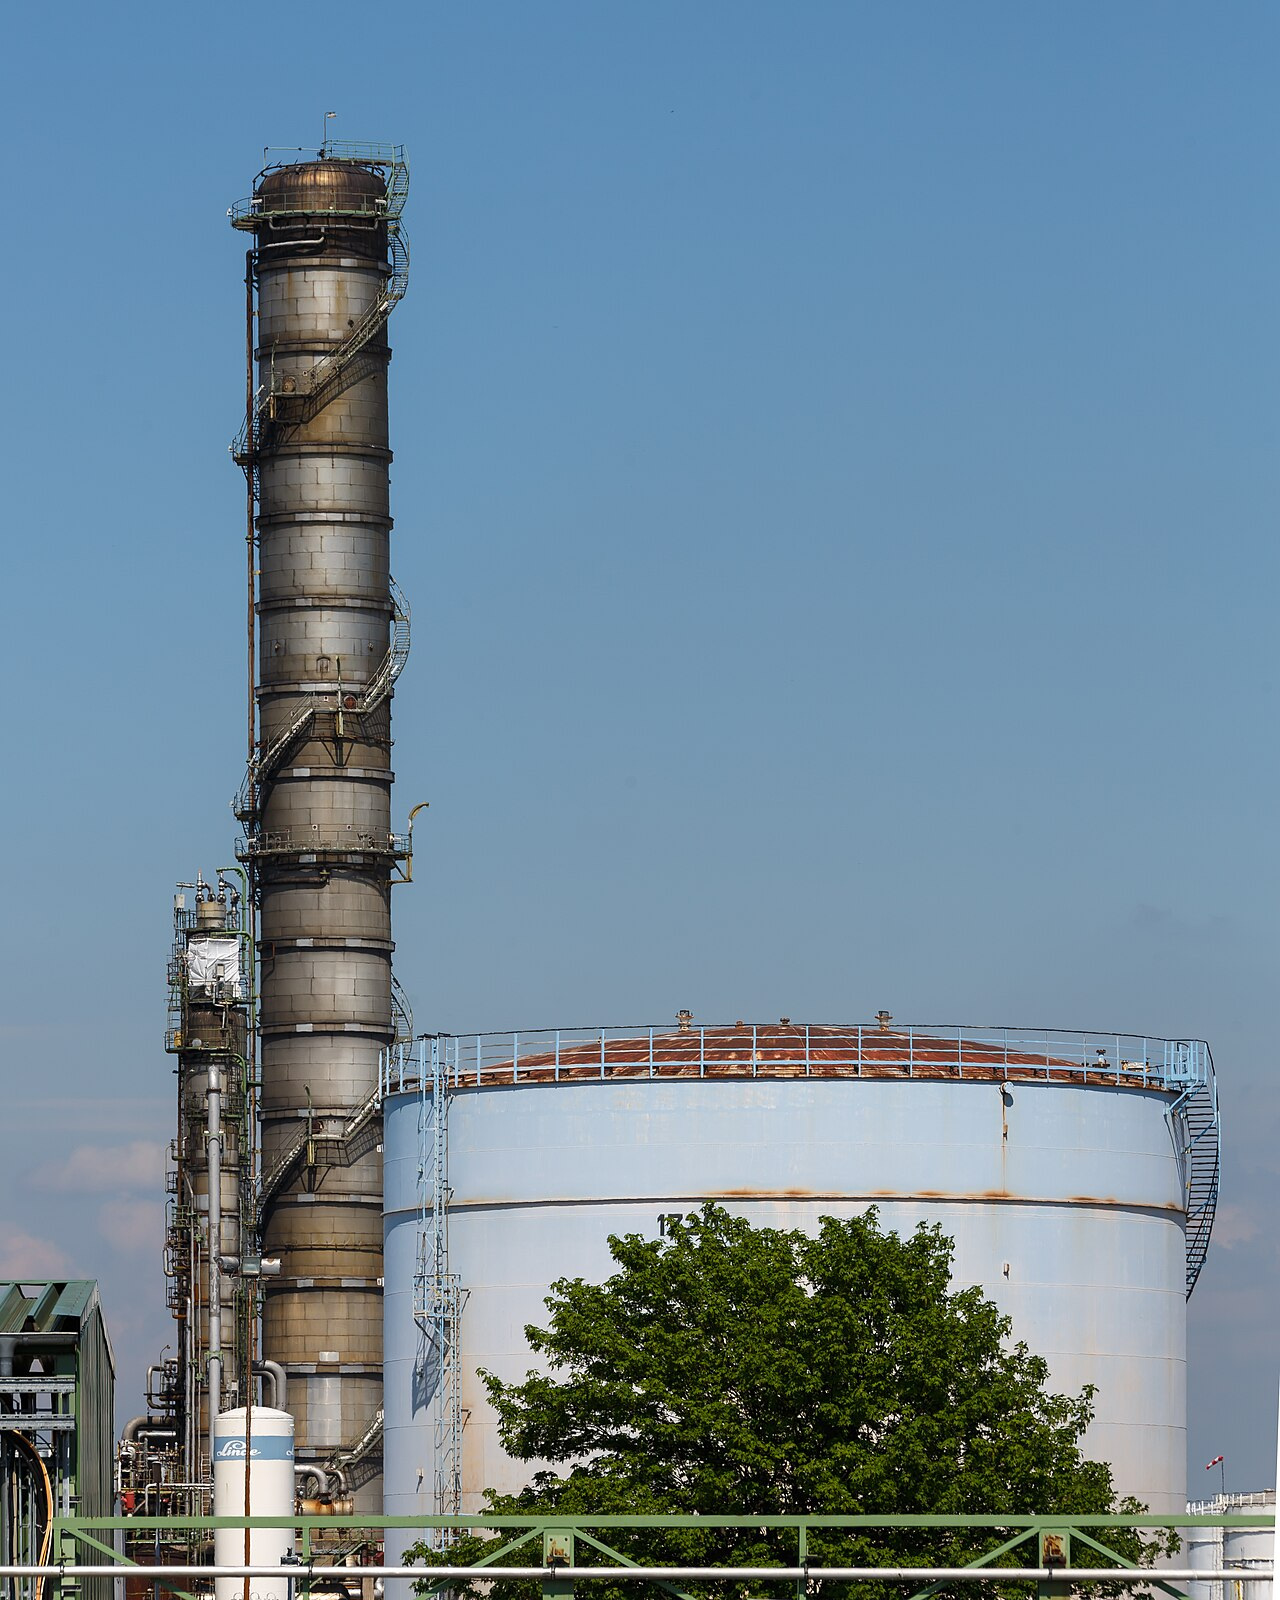
\includegraphics[width=\linewidth]{images/book3/refinery-column.jpg}
\end{minipage}

{\small يمينًا: عمود أطباق. يجري السائل عبر كل طبق ثم ينزل في
أنبوب الهبوط إلى الطبق الذي تحته؛ ويصعد البخار عبر الأطباق ويمر فقاعاتٍ
خلال السائل. ويُعاد جزء من البخار المكثَّف ارتدادًا؛ وتوفر
المِغلاة في القاع البخار. يسارًا: عمود تقطير في
مصفاة (كولونيا، 2014)، يضم عشرات الأطباق. (صورة: سي إي فوتو،
أوفه أراناس، CC~BY-SA~3.0، ويكيميديا كومنز.)}
\end{omfigure}

\begin{proposition}[فِنسكي]\label{prop:b2:liquid-vapour-diagrams:fenske}
عند الارتداد الكلي، ومع تطايرية نسبية ثابتة $\alpha$، يكون عدد
\omterm{def:b2:liquid-vapour-diagrams:fractional-distillation}{الأطباق النظرية} اللازم للانتقال من سائل قاع $x_B$ إلى قطير
$x_D$ على الأقل
\[
  N_{\min} = \frac{1}{\ln\alpha}\,\ln\!\left[\frac{x_D}{1 - x_D}\cdot\frac{1 - x_B}{x_B}\right] .
\]
\end{proposition}

\begin{proof}
نرقّم الأطباق من الأسفل، والمِغلاة هي الطبق 1. عند الارتداد الكلي
يكون للسائل النازل على الطبق $k + 1$ تركيب البخار
الخارج من الطبق $k$: $x_{k+1} = y_k$. ومع $r = x/(1 - x)$، يعطي كل طبق
$r(y_k) = \alpha\,r(x_k)$، ومنه $r(x_{k+1}) = \alpha\,r(x_k)$، وبعد $N$
طبقًا يكون للبخار المكثَّف $r(x_D) = \alpha^N r(x_B)$. وبأخذ اللوغاريتمات
نحصل على $N$. ومع ارتداد منتهٍ يكون السائل النازل أفقر من
البخار الصاعد، فيُغني كل طبق أقل، ويلزم مزيد من الأطباق.
\end{proof}

على المخطط $(x, y)$ يكون الإنشاء نفسه درجًا بين
منحنى التوازن والقطر $y = x$: كل درجة \omterm{def:b2:liquid-vapour-diagrams:fractional-distillation}{طبق نظري}
واحد.

\begin{omfigure}
\begin{tikzpicture}
\begin{axis}[width=0.55\linewidth, height=0.55\linewidth, xmin=0, xmax=1,
  ymin=0, ymax=1, axis x line=bottom, axis y line=left,
  xlabel={\shortstack{\foreignlanguage{arabic}{$x$ (البنزين، السائل)}}}, ylabel={\shortstack{\foreignlanguage{arabic}{$y$ (البنزين، البخار)}}},
  tick label style={font=\small}, label style={font=\small}]
\addplot[omThm, thick] table[x=x, y=y] {figdata/out/bachelor-2-liquid-vapour-f-eq.dat};
\addplot[black!50] coordinates {(0,0) (1,1)};
\addplot[omDef, thick] table[x=x, y=y] {figdata/out/bachelor-2-liquid-vapour-f.dat};
\draw[densely dotted] (axis cs:0.95,0) -- (axis cs:0.95,0.95);
\draw[densely dotted] (axis cs:0.05,0) -- (axis cs:0.05,0.05);
\node[font=\scriptsize, anchor=south east] at (axis cs:0.945,0.02) {$x_D$};
\node[font=\scriptsize, anchor=south west] at (axis cs:0.05,0.02) {$x_B$};
\end{axis}
\end{tikzpicture}

{\small الأطباق عند الارتداد الكلي للبنزين--التولوين، انطلاقًا من قطير
0.95 نزولًا: كل درجة أفقية تنتقل من بخار إلى السائل الذي في
توازن معه (طبق واحد)، وكل درجة عمودية من ذلك السائل إلى
بخار الطبق الذي تحته. سبع درجات تنزل بالسائل تحت $x_B = 0.05$؛
وتعطي صيغة فِنسكي 6.5.}
% ledger: antoine:benzene.A, antoine:toluene.A (computed in figdata/bachelor-2/liquid-vapour.py)
\end{omfigure}

\begin{proposition}[لا يستطيع العمود عبور أزيوتروب]\label{prop:b2:liquid-vapour-diagrams:azeotrope-limit}
في خليط فيه \omterm{def:b2:liquid-vapour-diagrams:azeotrope}{أزيوتروب}، يعطي العمود المغذّى من جهة من التركيب
الأزيوتروبي في أحسن الأحوال الأزيوتروبَ عند أحد طرفيه والمكوّن النقي
لتلك الجهة عند الطرف الآخر.
\end{proposition}

\begin{proof}
عند \omterm{def:b2:liquid-vapour-diagrams:azeotrope}{الأزيوتروب} يلاقي منحنى التوازن القطر: $y = x$. وقربه
تصير كل درجة من الدرج صغيرة جدًا، فلا يبلغه أي عدد منتهٍ من
الأطباق، ولا يعبره أي عدد.
\end{proof}

\begin{method}[التنبؤ بنتيجة تقطير تجزيئي]\label{met:b2:liquid-vapour-diagrams:predict-distillation}
\begin{enumerate}
  \item جِد أدنى نقطة غليان يمكن بلوغها من التغذية على
        \omterm{def:b2:liquid-vapour-diagrams:binary-diagram}{المخطط المتساوي الضغط}: مكوّن نقي أو \omterm{def:b2:liquid-vapour-diagrams:azeotrope}{أزيوتروب موجب}. فهي تخرج
        من القمة.
  \item وتبقى أعلى نقطة غليان في الجهة نفسها (مكوّن نقي أو
        \omterm{def:b2:liquid-vapour-diagrams:azeotrope}{أزيوتروب سالب}) في المغلاة.
  \item مع \omterm{def:b2:liquid-vapour-diagrams:azeotrope}{أزيوتروب}، انظر في أي جهة منه تقع التغذية: فلا يمكن الحصول إلا على
        المكوّن النقي لتلك الجهة.
  \item لعدد الأطباق، استعمل صيغة فِنسكي أو الدرج،
        ثم أضف أطباقًا من أجل الارتداد المنتهي المستعمل فعلًا.
\end{enumerate}
\end{method}

من أجل الإيثانول والماء المغذّيين بأقل من 0.881، تعطي القمة في أحسن الأحوال
الأزيوتروبَ والقاعُ الماءَ: فلا يعطي أي عمود إيثانولًا مطلقًا. وتجفيف
آخر جزء في المئة يتطلب طريقة أخرى --- منخلًا جزيئيًا يمتز الماء، أو
مكوّنًا ثالثًا يُضاف لكسر \omterm{def:b2:liquid-vapour-diagrams:azeotrope}{الأزيوتروب}.

\begin{omfigure}
\begin{tikzpicture}[font=\small, scale=0.95, >={Stealth}]
  \pic[transform shape] at (0,0) {heatingmantle};
  \pic[transform shape] at (0,0) {rbflask={0.45}{orange!25}};
  \foreach \x/\y in {-0.35/0.25,0.05/0.18,0.35/0.3}
    \fill[black!55] (\x,\y) circle (0.06);
  % Vigreux column from the flask neck (0,3) to (0,6)
  \draw[om glass] (-0.22,3.0) -- (-0.22,6.0) (0.22,3.0) -- (0.22,6.0);
  \foreach \yy in {3.4,3.9,4.4,4.9,5.4} {
    \draw[om glass] (-0.22,\yy) -- (-0.06,\yy+0.18) -- (-0.22,\yy+0.3);
    \draw[om glass] (0.22,\yy+0.15) -- (0.06,\yy+0.33) -- (0.22,\yy+0.45);
  }
  \pic[transform shape] (s) at (0,6.0) {stillhead};
  \pic[transform shape] at ($(s-top)+(0,-0.75)$) {thermometer};
  \pic[transform shape, rotate=-20] (c) at (s-arm) {liebig={3.4}};
  % ground-glass joint between the head's side arm and the condenser
  \draw[om glass, fill=white, rotate around={-20:(s-arm)}] ($(s-arm)+(-0.12,-0.17)$) rectangle ($(s-arm)+(0.14,0.17)$);
  \coordinate (cend) at ($(s-arm)+(-20:3.4)$);
  \pic[transform shape] (a) at (cend) {adapter};
  \pic[transform shape] at ($(a-tip)+(0,-2.4)$) {erlenmeyer={0.22}{orange!12}};
  \draw[<-, omProp, thick] (-0.25,4.6) -- (-1.6,4.6) node[left, text=black,
    align=right] {\shortstack[r]{\foreignlanguage{arabic}{عمود فيغرو}\\\foreignlanguage{arabic}{تجاويفه تضاعف}\\\foreignlanguage{arabic}{التلامسات}}};
  \draw[<-, omProp, thick] (0.12,6.72) -- (-1.4,7.4) node[left, text=black,
    align=right] {مستودع المحرار\\ بمستوى الذراع الجانبية};
  \draw[<-, omProp, thick] (1.08,0.3) -- (2.3,-0.2) node[right, text=black]
    {غلاف تسخين};
  \draw[<-, omProp, thick] ($(a-tip)+(0.75,-2.0)$) -- ++(1.0,0.2)
    node[right, text=black] {قطير};
\end{tikzpicture}

{\small \omterm{def:b2:liquid-vapour-diagrams:fractional-distillation}{التقطير التجزيئي} في المختبر. يؤدي عمود فيغرو بين
الدورق ورأس التقطير دور بضعة \omterm{def:b2:liquid-vapour-diagrams:fractional-distillation}{أطباق نظرية}: يتكثف البخار
على تجاويفه ويعود فيتبخر في صعوده. وتبقى درجة
الحرارة عند الرأس عند درجة غليان المكوّن الأكثر تطايرًا ما دام
يتقطر، ثم ترتفع.}
\end{omfigure}

\begin{inthelab}[فصل سائلين بالتقطير التجزيئي]
يُملأ الدورق إلى نصفه على الأكثر، مع حصى الغليان، ويُسخَّن بلطف
بحيث تصعد حلقة البخار المتكثف في العمود ببطء: فالعمود الذي
يُغرقه التسخين السريع يفقد أطباقه. وتُسجَّل درجة حرارة الرأس كل
بضعة مليلترات؛ ويُغيَّر المستقبِل حين تبدأ بالارتفاع (فتُجمع
\textit{قطفة} عند كل درجة من درجات الحرارة)، ويُوقف التسخين
قبل أن يجف الدورق.
\end{inthelab}

\section{السوائل الجزئية الامتزاج وغير القابلة للامتزاج}

\begin{definition}[فجوة الامتزاج]\label{def:b2:liquid-vapour-diagrams:miscibility-gap}
\emph{فجوة الامتزاج}\index{فجوة الامتزاج} هي مجال التراكيب
الإجمالية الذي ينفصل فيه سائلان، عند درجة حرارة معيّنة، إلى طبقتين
سائلتين، كل منهما مشبعة بالمكوّن الآخر. و\emph{الأزيوتروب
غير المتجانس}\index{أزيوتروب غير متجانس} هو نقطة غليان سائل كهذا ذي
طبقتين: تتعايش فيه الطبقتان السائلتان والبخار عند درجة حرارة ثابتة
وبتركيب ثابت للبخار.
\end{definition}

عند \omterm{def:b2:liquid-vapour-diagrams:miscibility-gap}{الأزيوتروب غير المتجانس} يكون مكوّنان في ثلاثة أطوار: فعند ضغط ثابت
تكون \omterm{def:b2:equilibrium-shifts:variance}{التغايرية} $2 + 2 - 3 - 1 = 0$. فتبقى درجة الحرارة
ثابتة، كما عند نقطة غليان سائل نقي، ما دامت الطبقتان
موجودتين.

\begin{omfigure}
\begin{tikzpicture}[font=\small, x=6cm, y=0.08cm]
  \draw[->] (0,0) -- (1.05,0) node[right] {$x$};
  \draw[->] (0,0) -- (0,62) node[above] {$T$};
  \node[below] at (0,0) {2}; \node[below] at (1,0) {1};
  % boiling points: 2 at 50, 1 at 42; heteroazeotrope at 25 with layers 0.1 and 0.85, vapour 0.6
  \draw[omliquidus] (0,50) .. controls (0.04,38) and (0.08,30) .. (0.1,25);
  \draw[omliquidus] (1,42) .. controls (0.95,34) and (0.9,28) .. (0.85,25);
  \draw[omsolidus] (0,50) .. controls (0.25,46) and (0.5,35) .. (0.6,25);
  \draw[omsolidus] (1,42) .. controls (0.9,37) and (0.7,30) .. (0.6,25);
  \draw[thick] (0.1,25) -- (0.85,25);
  \draw[omliquidus] (0.1,25) -- (0.07,2);
  \draw[omliquidus] (0.85,25) -- (0.9,2);
  \fill (0.6,25) circle[radius=2pt];
  \node[font=\scriptsize] at (0.47,6) {طبقتان سائلتان};
  \node[font=\scriptsize] at (0.5,55) {بخار};
  \node[font=\scriptsize] at (0.035,12) {L$_2$};
  \node[font=\scriptsize] at (0.96,12) {L$_1$};
  \node[font=\scriptsize, align=center] at (0.3,33) {\babelsublr{L$_2$ + V}};
  \node[font=\scriptsize, anchor=west] at (1.06,36) {\babelsublr{L$_1$ + V}};
  \draw[thin] (1.06,36) -- (0.86,29.5);
  \node[font=\scriptsize, anchor=north] at (0.6,24) {أزيوتروب غير متجانس};
\end{tikzpicture}

{\small مخطط تخطيطي متساوي الضغط لسائلين جزئيي الامتزاج. تحت
درجة حرارة \omterm{def:b2:liquid-vapour-diagrams:miscibility-gap}{الأزيوتروب غير المتجانس} ينقسم السائل إلى طبقتين L$_1$ 
وL$_2$ على مجال واسع من التراكيب (\omterm{def:b2:liquid-vapour-diagrams:miscibility-gap}{فجوة الامتزاج})؛ وعلى
الخط الأفقي تغلي الطبقتان معًا معطيتين بخارًا ثابت
التركيب (النقطة).}
\end{omfigure}

\begin{definition}[التقطير ببخار الماء]\label{def:b2:liquid-vapour-diagrams:steam-distillation}
\emph{التقطير ببخار الماء}\index{تقطير ببخار الماء} هو تقطير
سائل غير قابل للامتزاج بالماء بنفخ بخار الماء عبره: فيغلي الخليط
تحت درجة غليان كلا السائلين، وينفصل القطير إلى
طبقتين.
\end{definition}

لا يختلف \omterm{def:b2:liquid-vapour-diagrams:steam-distillation}{التقطير ببخار الماء} عن التقطير المائي في المجلد المدرسي
إلا في طريقة إدخال الماء: بخار ينفخ عبر المادة، بدل
مادة تغلي في الماء. والترموديناميك واحد.

\begin{proposition}[غليان سائلين غير قابلين للامتزاج]\label{prop:b2:liquid-vapour-diagrams:steam}
يغلي سائلان غير قابلين للامتزاج متلامسان عند درجة الحرارة التي يساوي فيها مجموع
ضغطي بخارهما الضغط الخارجي، $p_1^*(T) + p_2^*(T) =
p$، وهي أدنى من درجتي غليانهما. ويحوي القطير السائلين
بنسبة الكتلتين
\[
  \frac{m_1}{m_2} = \frac{p_1^*\,M_1}{p_2^*\,M_2} .
\]
\end{proposition}

\begin{proof}
كل سائل نقي يبذل ضغط بخاره الخاص، أيًّا كانت كمية
الآخر: فالضغط الكلي فوق الطبقتين هو $p_1^* + p_2^*$، الذي
يبلغ $p$ عند درجة حرارة يكون فيها كل $p_i^*$ أصغر من $p$. وفي
البخار تتناسب كميات المادة مع الضغوط الجزئية، $n_1/n_2 =
p_1^*/p_2^*$؛ نضرب في $M_1/M_2$.
\end{proof}

\begin{omfigure}
\begin{tikzpicture}
\begin{axis}[width=0.6\linewidth, height=5.5cm, xmin=70, xmax=100, ymin=0, ymax=1.6,
  axis x line=bottom, axis y line=left, xlabel={\babelsublr{$T$ (\unit{\degreeCelsius})}},
  ylabel={\babelsublr{$p$ (\unit{bar})}}, tick label style={font=\small},
  label style={font=\small}, clip=false]
\addplot[omProp, thick] table[x=t, y=ptol] {figdata/out/bachelor-2-liquid-vapour-e.dat};
\addplot[omDef, thick] table[x=t, y=pwat] {figdata/out/bachelor-2-liquid-vapour-e.dat};
\addplot[black, very thick] table[x=t, y=psum] {figdata/out/bachelor-2-liquid-vapour-e.dat};
\draw[densely dashed] (axis cs:70,1.013) -- (axis cs:100,1.013) node[right, font=\scriptsize] {\qty{1.013}{bar}};
\draw[densely dotted] (axis cs:84.3,0) -- (axis cs:84.3,1.013);
\node[font=\scriptsize, anchor=south east] at (axis cs:84.3,1.05) {\qty{84.3}{\degreeCelsius}};
\node[font=\scriptsize, anchor=west] at (axis cs:96,1.45) {المجموع};
\node[font=\scriptsize, omDef, anchor=south] at (axis cs:77,0.46) {الماء};
\node[font=\scriptsize, omProp, anchor=north west] at (axis cs:88,0.5) {التولوين};
\end{axis}
\end{tikzpicture}

{\small التولوين والماء، غير القابلين للامتزاج: ضغطا بخار كل سائل
ومجموعهما. تغلي الطبقتان معًا عند \qty{84.3}{\degreeCelsius}، تحت
درجة غليان الماء (\qty{100}{\degreeCelsius}) والتولوين (\qty{110.6}{\degreeCelsius})؛
ويحمل القطير 4.1 غ من التولوين لكل غرام من الماء.}
% ledger: antoine:toluene.A, antoine:water.A, aw:C, aw:H, aw:O (computed in figdata/bachelor-2/liquid-vapour.py)
\end{omfigure}

تتقطر بهذه الطريقة الجزيئات الثقيلة الهشة للزيوت العطرية النباتية عند ما يقل
بقليل عن \qty{100}{\degreeCelsius}، أي أدنى بكثير من درجات غليانها الخاصة، مع
قليل من التفكك؛ والثمن قطير أغلبه ماء.

\section{تمارين}

\begin{exercise}[$\star$]\label{exo:b2:liquid-vapour-diagrams:1}
على \omterm{def:b2:liquid-vapour-diagrams:binary-diagram}{المخطط المتساوي الضغط} للبنزين--التولوين، اقرأ درجتي غليان السائلين
النقيين، \omterm{def:b2:liquid-vapour-diagrams:bubble-dew}{ونقطة الفقاعة} لسائل تركيبه 0.2 وتركيب
أول بخار له.
\end{exercise}

\begin{exercise}[$\star$]\label{exo:b2:liquid-vapour-diagrams:2}
عند \qty{80}{\degreeCelsius} يكون ضغطا بخار البنزين والتولوين
\qty{1.010}{bar} و\qty{0.388}{bar}. احسب، لسائل متساوي المولات،
الضغط الذي يبدأ عنده بالغليان وتركيب البخار.
\end{exercise}

\begin{exercise}[$\star$]\label{exo:b2:liquid-vapour-diagrams:3}
يوجد \qty{10}{mol} من خليط تركيبه الإجمالي 0.30 عند درجة حرارة
يكون فيها تركيب السائل 0.20 وتركيب البخار 0.45. احسب كميتي
الطورين.
\end{exercise}

\begin{exercise}[$\star$]\label{exo:b2:liquid-vapour-diagrams:4}
احسب \omterm{def:b2:equilibrium-shifts:variance}{تغايرية} خليط بنزين--تولوين (أ) سائل كله؛ (ب)
يغلي؛ (ج) عند \omterm{def:b2:liquid-vapour-diagrams:azeotrope}{أزيوتروب}، لزوج له \omterm{def:b2:liquid-vapour-diagrams:azeotrope}{أزيوتروب}، عند ضغط ثابت.
\end{exercise}

\begin{exercise}[$\star\star$]\label{exo:b2:liquid-vapour-diagrams:5}
جِد بالتجربة والخطأ \omterm{def:b2:liquid-vapour-diagrams:bubble-dew}{نقطة الندى} لبخار بنزين--تولوين تركيبه 0.30 عند
\qty{1.013}{bar}، مستعملًا $p^*_{\text{بنزين}}$ و$p^*_{\text{تولوين}}$
(\unit{bar}): 1.80 و0.742 عند \qty{100}{\degreeCelsius}، و2.057 و0.861 عند
\qty{105}{\degreeCelsius}. وأعطِ تركيب أول قطرة.
\end{exercise}

\begin{exercise}[$\star\star$]\label{exo:b2:liquid-vapour-diagrams:6}
يُقطَّر خليط بنزين--تولوين متساوي المولات تقطيرًا بسيطًا (دون عمود). ما
تركيب أول قطرات القطير؟ وكيف تتغير درجة الحرارة وتركيب
القطير مع تقدم التقطير؟ ولماذا يكون
الفصل رديئًا؟
\end{exercise}

\begin{exercise}[$\star\star$]\label{exo:b2:liquid-vapour-diagrams:7}
يُقطَّر نبيذ كسره المولي من الإيثانول 0.05 تقطيرًا تجزيئيًا بعمود شديد
الكفاءة. ماذا يخرج من القمة، وماذا يبقى في المغلاة؟
والسؤال نفسه لخليط كسره المولي 0.95.
\end{exercise}

\begin{exercise}[$\star\star$]\label{exo:b2:liquid-vapour-diagrams:8}
لمكوّن من زيت عطري نباتي (كتلته المولية \qty{136}{g/mol}) ضغط بخار
قدره \qty{0.10}{bar} قرب \qty{97}{\degreeCelsius}، حيث ضغط بخار الماء
\qty{0.91}{bar} (معطيات التمرين). عند أي درجة حرارة يجري \omterm{def:b2:liquid-vapour-diagrams:steam-distillation}{التقطير ببخار الماء}
تحت \qty{1.013}{bar}، وكم غرامًا من الزيت العطري
يُجمع لكل غرام من الماء؟
\end{exercise}

\begin{exercise}[$\star\star$]\label{exo:b2:liquid-vapour-diagrams:9}
على المخطط التخطيطي للسائلين الجزئيي الامتزاج، صِف ما يحدث
حين يُسخَّن خليط ذو طبقتين تركيبه الإجمالي 0.4 من درجة حرارة الغرفة
حتى يصير كله بخارًا: الأطوار، ودرجات الحرارة، وتركيب
أول بخار.
\end{exercise}

\begin{exercise}[$\star\star\star$]\label{exo:b2:liquid-vapour-diagrams:10}
مع $\alpha = 2.47$، احسب العدد الأدنى من \omterm{def:b2:liquid-vapour-diagrams:fractional-distillation}{الأطباق النظرية} لقطير
تركيبه 0.99 وقاع تركيبه 0.01. وقارن بالعدد 6.5 اللازم للتركيبين 0.95
و0.05، وعلّق على كلفة النقاوة.
\end{exercise}

\begin{exercise}[$\star\star\star$]\label{exo:b2:liquid-vapour-diagrams:11}
انطلاقًا من \omterm{def:b2:liquid-vapour-diagrams:binary-diagram}{المخطط المتساوي الضغط} للبنزين--التولوين ومن معادلتي أنطوان،
فسّر كيف يُحصل على \omterm{def:b2:liquid-vapour-diagrams:binary-diagram}{المخطط المتساوي الحرارة} عند \qty{80}{\degreeCelsius}،
ولماذا تقع عليه منطقة السائل في الأعلى.
\end{exercise}

\begin{exercise}[$\star\star\star$]\label{exo:b2:liquid-vapour-diagrams:12}
انطلاقًا من العلاقة $d\ln p = (y - x)\,dy/[y(1 - y)]$، بيّن أن الضغط الكلي يتزايد
عند درجة حرارة ثابتة مع $x$ حيثما كان البخار أغنى من السائل بالمكوّن 1،
واستنتج أن \omterm{def:b2:chemical-potential:ideal-mixture}{الخليط المثالي} لا \omterm{def:b2:liquid-vapour-diagrams:azeotrope}{أزيوتروب} له.
\end{exercise}

\section{مسألة: عمود للبنزين والتولوين}

\begin{problem}[{مسألة نهاية الأسبوع --- المخطط المتساوي الضغط للبنزين
والتولوين من معادلتي أنطوان، وتبخير فجائي وقاعدة الرافعة، والعدد الأدنى
من أطباق عمود عند الارتداد الكلي، والحد الذي يفرضه
أزيوتروب}]
\label{pb:b2:liquid-vapour-diagrams:1}
المعطيات: معادلتا أنطوان، $\log_{10}(p^*/\unit{bar}) = A - B/(T + C)$ مع $T$
بالكلفن: البنزين $A = 4.01814$، $B = \qty{1203.835}{K}$، $C =
\qty{-53.226}{K}$؛ والتولوين $A = 4.07827$، $B = \qty{1343.943}{K}$، $C =
\qty{-53.773}{K}$. الضغط \qty{1.013}{bar}؛ ويكوّن البنزين والتولوين \omterm{def:b2:chemical-potential:ideal-mixture}{خليطًا
مثاليًا}. ويحوي \omterm{def:b2:liquid-vapour-diagrams:azeotrope}{أزيوتروب} الإيثانول--الماء 95~\% من الإيثانول كتلةً.
% ledger: antoine:benzene.A, antoine:benzene.B, antoine:benzene.C, antoine:toluene.A, antoine:toluene.B, antoine:toluene.C, azeo:ethanol-water.w

\medskip
\noindent\textbf{الجزء الأول --- المخطط.}
\begin{enumerate}
  \item احسب درجتي غليان البنزين والتولوين عند \qty{1.013}{bar}.
  \item احسب $p_1^*$ و$p_2^*$ عند \qty{90}{\degreeCelsius}.
  \item استنتج تركيبي السائل والبخار في توازن
        عند \qty{90}{\degreeCelsius}.
  \item السؤال نفسه عند \qty{100}{\degreeCelsius} ($p_1^* = \qty{1.800}{bar}$، $p_2^* =
        \qty{0.742}{bar}$).
  \item ارسم بخطوط تقريبية \omterm{def:b2:liquid-vapour-diagrams:binary-diagram}{المخطط المتساوي الضغط} انطلاقًا من هذه النقاط الأربع ومن السائلين النقيين.
  \item جِد \omterm{def:b2:liquid-vapour-diagrams:bubble-dew}{نقطة الفقاعة} لسائل متساوي المولات، بدقة
        \qty{0.5}{\degreeCelsius}، بالتجربة والخطأ بين \qty{90}{\degreeCelsius} 
        و\qty{95}{\degreeCelsius}.
  \item احسب \omterm{def:b2:equilibrium-shifts:variance}{تغايرية} الخليط الذي يغلي وبيّن ما تعنيه
        للمخطط.
\end{enumerate}

\medskip
\noindent\textbf{الجزء الثاني --- تبخير فجائي.}
\begin{enumerate}[resume]
  \item تُسخَّن تغذية متساوية المولات إلى \qty{95}{\degreeCelsius} ($p_1^* =
        \qty{1.569}{bar}$، $p_2^* = \qty{0.636}{bar}$). احسب $x$ و$y$.
  \item من أجل \qty{100}{mol} من التغذية، احسب كميتي السائل والبخار.
  \item احسب كمية البنزين في كل طور وتحقق من الحصيلة.
  \item ما كسر البنزين المسترجَع في البخار؟
  \item ماذا يحدث إذا أُجري التبخير الفجائي عند \qty{100}{\degreeCelsius}؟
  \item عند أي درجة حرارة تتبخر التغذية كلها؟
\end{enumerate}

\medskip
\noindent\textbf{الجزء الثالث --- العمود.}
\begin{enumerate}[resume]
  \item عرّف التطايرية النسبية $\alpha$ واحسبها عند درجة
        غليان البنزين.
  \item احسبها عند درجة غليان التولوين.
  \item خذ المتوسط الهندسي قيمةً للعمود كله.
  \item بيّن أنه على \omterm{def:b2:liquid-vapour-diagrams:fractional-distillation}{طبق نظري} $y/(1 - y) = \alpha\,x/(1 - x)$.
  \item فسّر لماذا يكون للسائل الداخل إلى طبق، عند الارتداد الكلي،
        تركيب البخار الخارج من الطبق الذي تحته.
  \item استنتج صيغة فِنسكي.
  \item احسب العدد الأدنى من \omterm{def:b2:liquid-vapour-diagrams:fractional-distillation}{الأطباق النظرية} لقطير تركيبه
        0.95 وقاع تركيبه 0.05.
  \item لماذا يُعطى العمود الحقيقي أطباقًا أكثر من ذلك؟
  \item على درج الفصل، عدّ الدرجات وقارن.
\end{enumerate}

\medskip
\noindent\textbf{الجزء الرابع --- \omterm{def:b2:liquid-vapour-diagrams:azeotrope}{أزيوتروب}.}
\begin{enumerate}[resume]
  \item احسب الكسر المولي للإيثانول في \omterm{def:b2:liquid-vapour-diagrams:azeotrope}{أزيوتروب} الإيثانول--الماء.
  \item تدخل تغذية فيها 0.10 من الإيثانول عمودًا من خمسين طبقًا. ماذا يخرج
        من القمة ومن القاع؟
  \item اذكر العدد الأدنى من \omterm{def:b2:liquid-vapour-diagrams:fractional-distillation}{الأطباق النظرية} اللازم لفصل
        البنزين والتولوين إلى ناتجين نقاوة كل منهما 95~\%.
\end{enumerate}
\end{problem}
